\documentclass[11pt]{article}
\usepackage[a4paper,margin=22mm]{geometry}
\usepackage{graphicx}
\usepackage{booktabs}
\usepackage{tabularx}
\usepackage{url}
\usepackage[hidelinks]{hyperref}
\newcommand{\code}[1]{\texttt{#1}}
\newcommand{\OLV}{OpenLiDARViewer}
\usepackage{caption}
\usepackage{newtxtext,newtxmath}
\usepackage{microtype}
\pagestyle{empty}
\begin{document}
\begin{center}
{\Large\bfseries Evidence-Monotone Terrain Representation (EMTRF)}\\[4pt]
{\large Supplementary Material}
\end{center}
\vspace{6mm}

\begin{table}[h]
\centering
\caption*{\textbf{Table S1.} Descriptive DTM support structure used to interpret site heterogeneity (referenced from the main-text ``Interpreting site heterogeneity'' discussion). Cell fractions are over each frozen crop. ``M/I edge'' is the fraction of horizontal/vertical adjacent supported-cell pairs with different measured/interpolated ancestry. These are post-hoc mechanism diagnostics, not causal terrain effects.}
\vspace{2mm}
\small
\setlength{\tabcolsep}{6pt}
\begin{tabular}{@{}lrrrrrr@{}}
\toprule
Site & $M$ cells & $I$ cells & $U$ cells & Median $n_M$ & M/I edge & $M$ dashed \\
\midrule
White Sands & 35.2\% & 32.8\% & 32.0\% & 12 & 0.94\% & 32.3\% \\
Estonia Tava & 76.3\% & 23.7\% & 0.0\% & 2 & 29.60\% & 50.6\% \\
StREAM & 66.9\% & 33.1\% & 0.0\% & 2 & 29.33\% & 59.8\% \\
Marsh Island & 0.8\% & 50.3\% & 48.9\% & 41 & 0.80\% & 15.5\% \\
\bottomrule
\end{tabular}
\end{table}

\vspace{8mm}

\begin{table}[h]
\centering
\caption*{\textbf{Table S2.} Site-specific four-pipeline ablation and performance diagnostics at one source-cell tolerance (the per-site detail behind the main-text P0--P3 ablation summary table). ``EP promote'' is the endpoint-only rate shared by P0/P1; ``Grade loss'' is the rate shared by P0/P2; ``Typed-EP loss'' is P1. The P3 column reports support-promotion/provenance-loss counts. The EC-DP overhead per kilometre is a secondary microtiming diagnostic; the paired 5,305-vertex benchmark in the main text is the primary runtime estimate.}
\vspace{2mm}
\small
\setlength{\tabcolsep}{5pt}
\begin{tabular}{@{}lrrrrrrr@{}}
\toprule
Site & Spans & Red. & EP promote & Grade loss & Typed-EP loss & P3 & +ms/km \\
\midrule
White Sands & 82 & 71.1\% & 24.4\% & 93.9\% & 0.0\% & 0/0 & 2.12 \\
Estonia Tava & 172 & 62.7\% & 6.4\% & 100\% & 7.6\% & 0/0 & 2.43 \\
StREAM & 54 & 67.4\% & 22.2\% & 100\% & 1.9\% & 0/0 & 2.05 \\
Marsh Island & 184 & 87.5\% & 4.3\% & 98.9\% & 0.0\% & 0/0 & 2.78 \\
\bottomrule
\end{tabular}
\end{table}

\vspace{8mm}

\begin{figure}[h]
\centering
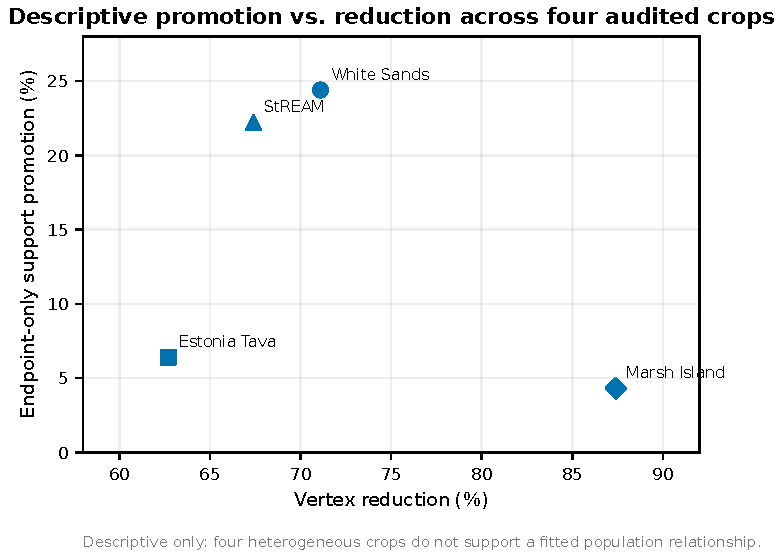
\includegraphics[width=0.86\linewidth]{supplementary/figS1_promotion_vs_reduction.pdf}
\caption*{\textbf{Figure S1.} Descriptive endpoint-only support-promotion rate versus vertex reduction at one source-cell tolerance for the four audited field-derived crops. The points summarize heterogeneous crops and are shown only to expose the joint range of simplification and evidence failure. No fitted population relationship or causal association is claimed.}
\end{figure}

\clearpage
\section*{Supplementary Methods}

\noindent\textbf{S1. Adversarial source-arc fixtures.} For each $\varepsilon\in\{0.02,0.05,0.10,0.20,0.40\}$, 2{,}000 deterministic 64-vertex polylines were generated from a low-amplitude sinusoidal geometry with a fixed mulberry32 seed family (seed \texttt{0xC0FFEE}$+$index). Source supports were sampled from $[0.78,0.98)$; one to four non-endpoint vertices were then replaced by weak support in $[0.08,0.50)$. Ordinary DP and EC-DP used the same geometric recursion. For every simplified span the endpoint-only value was the minimum of its retained endpoints, and the contract value was the minimum across the complete represented source arc; an endpoint-only promotion was counted when the former exceeded the latter, and a geometry mismatch when the retained index sets differed on fully supported fixtures. A separate gap experiment generated 1{,}000 fixtures, marked one interior vertex unsupported, and simplified at $\varepsilon=0.25$; a baseline bridge was a DP segment whose retained endpoints lay on opposite sides of the unsupported vertex, whereas EC-DP split the source at that vertex so any crossing segment would violate the contract. A closed-ring extension used a deterministic 32-vertex ring with one weak interior value: when no semantic boundary supplies a start, the reference rule selects the lexicographically smallest $(x,y)$ vertex, rotates the ring to that anchor, duplicates it to unroll the cycle, applies EC-DP, and re-closes the output, with complete-source evidence including the cyclic interval adjacent to the cut. All 32 cyclic reindexings were required to produce one canonical output signature.

\vspace{4mm}
\noindent\textbf{S2. Real-data block-recovery audit.} For each executed crop the study called the frozen production rasterization, confidence-aware DTM, and contour modules. Each emitted marching-squares segment lies within one known $2\times2$ DTM-cell block; the audit recovered that producing block geometrically and required its recomputed four-corner minimum confidence to match the emitted segment confidence. Source provenance was reconstructed from the four cell states, stored independently of visual grade: $M$ when all four cells were measured-derived, $I$ when all four were interpolated-derived, and $X$ when both occurred. Unsupported corners cannot produce a segment because the contour extractor already refuses such cells.

\vspace{4mm}
\noindent\textbf{S3. Standalone study components.} The study is independent of the production application. It contains a JavaScript implementation of the reference support functions, directional classifier, ordinary DP, EC-DP, deterministic fixture generation, unsupported-gap injection, cyclic-ring handling, and timing harness. One independently written Python oracle checks the typed-evidence algebra, including the applicability, scope and lineage clauses: a channel that is not applicable to a source is ignored, whereas a channel applicable to a required source but carrying no value makes the output channel unavailable rather than computed from the remaining sources (a refusal preserved under composition), output scope is the intersection of the applicable sources' scopes, and lineage is the complete union over the source set. The same six clauses are also asserted against the shipped implementation by the exact conformance checks; a second Python program independently reimplements ordinary DP and EC-DP and is evaluated differentially on the same deterministic fixture coordinates and supports rather than by calling JavaScript output. Raw results, environment metadata, and checksums are frozen with the study artifacts.

\vspace{4mm}
\noindent\textbf{S4. Timing protocol.} For the synthetic benchmark, after five warm-ups ordinary DP and EC-DP were timed in 30 paired repetitions with alternating execution order, and retained-geometry checksums were required to match. The four-site real-contour benchmark used a site-normalized tolerance of one source grid cell (1.0 m for White Sands, Estonia Tava, and StREAM; 0.5 m for Marsh Island) over 289 polylines and 5{,}305 source vertices per pass; because one pass is sub-millisecond, each timed repetition batched 100 identical passes with five warm-ups and 30 alternating paired repetitions, then divided by 100. This is a post-contour representation-stage benchmark and excludes point loading, DTM construction, contour extraction, browser rendering, and GPU work.

\vspace{4mm}
\noindent\textbf{S5. Excluded context crop.} A USGS Coconino 3DEP context crop was executable but yielded only one stitched polyline and seven contour segments, too few for site-level quantitative comparison, and is therefore excluded from the quantitative corpus.

\vspace{8mm}

\noindent\textbf{Supplementary source audit.} The grade-to-label export mapping audited in the main text
(\texttt{solid}\,$\rightarrow$\,\texttt{measuredBacked}, \texttt{dashed}\,$\rightarrow$\,\texttt{interpolatedBacked})
is present in the audited OpenLiDARViewer source. The canonical archive is the v0.6.5 release at git commit
\texttt{4fb00a784d860a2e24cc1834d6c1230dac550355} (version {DOI} 10.5281/zenodo.21933671, source-archive SHA-256
\texttt{fdb510e3416fb0cb02c71031bb7f653b8e0dde83ae9916c85d1c44e844b122fa}). The identical mapping also appears
unchanged in earlier v0.6.4 development snapshots (2026-08-09, SHA-256
\texttt{71507a5115de8c8ad9125215e30222d87ca1cd400308fd464cebaac269373aaf} and
\texttt{1dfe94ef79838772730a04df66037b973a7be6b42abeecbf6f6ad7d6fd6c145f}), confirming the counterexample is a
stable export design carried across versions rather than a transient state of one archive.

\vspace{3mm}
\noindent\emph{Module reachability and test coverage.} The shipped \texttt{simplifyPolyline} path pins vertices below the
solid-confidence floor and vertices adjacent to grade transitions. The separate \texttt{contourAdaptiveGeneralize.ts}
module likewise delegates geometry to per-feature DP, but its own source documentation states it has no production
caller, so replacing that module alone would not make exported contour evidence conformant. In the updated test tree,
evidence-registry and evidence-monotonicity tests reject authority upgrades in registered derivation chains and the E4
studies check selected numerical operators, whereas the adaptive-generalization tests exercise tolerance selection and
geometry immutability/retention, not complete-source provenance/support serialization. Test reachability and operator
conformance are therefore separate claims.


\vspace{4mm}
\noindent\textbf{S6. Cross-implementation validation context (E4).} The audited source defines E4 as agreement with a second implementation of the same computation, separate from E5 field ground truth. Two E4 records bear on the upstream geometry used in the main text: the mean 1~m DTM on the Estonia crop against a NumPy point-in-cell mean, and marching-squares isolines against GDAL on an analytic DEM. Both are author-run implementation-agreement cross-checks, not evidence that export provenance is correct, and not field-accuracy validation.

\clearpage
\begin{table}[h]
\centering
\caption*{\textbf{Table S3.} Notation summary for the EMTRF contract (main-text Section 2).}
\vspace{2mm}
\small
\setlength{\tabcolsep}{4pt}
\begin{tabularx}{\linewidth}{@{}lX@{}}
\toprule
Symbol & Meaning \\
\midrule
$e_i=(p_i,S_i,A_i,\ell_i)$ & evidence record for cell $i$ \\
$p_i\subseteq\{M,I\}$ & provenance: measured-derived $M$, interpolated-derived $I$; mixed $X=\{M,I\}$ \\
$U$ & unsupported state: no authorized supported elevation (absorbing) \\
$S_i$ & typed support map, semantic channel $\mapsto[0,1]$ \\
$A_i$ & applicability and scientific scope of each support channel \\
$\ell_i$ & source lineage \\
$\mu$ & a semantic support channel (e.g.\ \texttt{measured-support}) \\
$D_y$; $D_y^{\mu}$ & complete required source set for output $y$; its subset for which $\mu$ is applicable \\
$S_y(\mu)=\min_{x\in D_y^{\mu}}S_x(\mu)$ & same-channel meet \\
$C_M(n;n_t,h)$; $C_I(d,\rho,\gamma)$ & reference measured / interpolated support profiles \\
$p_j^{\mathrm{EC}}$; $S_j^{\mathrm{EC}}(\mu)$ & EC-DP provenance union and support meet over the complete replaced arc \\
$n$; $m$; $\varepsilon$ & source vertices; retained segments; Douglas--Peucker tolerance \\
\bottomrule
\end{tabularx}
\end{table}

\vspace{6mm}
\section*{Supplementary Notes}

\noindent\textbf{N1. Worked substitution of the reference support profile.} The measured and interpolated
reference support functions (main-text Eqs.~3--4) are conformance profiles, not part of the EMTRF contract, and
may be replaced by any monotone support model without affecting provenance, applicability, lineage, or EC-DP
geometry. As a concrete example, suppose an interpolation method supplies a kriging standard error $\sigma_K$ and
defines a new typed channel $S_K=\sigma_0/(\sigma_0+\sigma_K)$ with $\sigma_0>0$, applicable only to
interpolated-derived cells. For $\sigma_0=0.25$~m and a source arc with $\sigma_K=\{0.10,0.25,0.40\}$~m, the
channel values are approximately $\{0.714,0.500,0.385\}$ and the representation-only meet is $0.385$. Replacing the
cell-level formula changes only how that typed channel is built; the provenance union, unsupported absorption,
applicability, lineage, and EC-DP geometry are unchanged. This substitutability is why the reported mechanism
failures do not depend on the particular numerical support scale.


\clearpage
\begin{table}[h]
\centering
\caption*{\textbf{Table S4.} Source context for the four field-derived contour crops. Metadata are limited to the fields frozen in the current OLV terrain-field and dataset manifests; ``not frozen'' means the committed crop records campaign/year context but not an exact flight day or instrument model. Checkpoints, where present, are not used to validate the EMTRF representation invariant.}
\vspace{2mm}
\small
\scriptsize
\setlength{\tabcolsep}{3.0pt}
\begin{tabularx}{\linewidth}{@{}p{0.17\linewidth}p{0.25\linewidth}p{0.30\linewidth}p{0.20\linewidth}@{}}
\toprule
Crop & Acquisition / platform & Instrument and committed crop context & CRS / vertical reference \\
\midrule
White Sands & 2020 USGS 3DEP airborne LiDAR & Optech Galaxy; gypsum-dune ground crop derived from source tile \nolinkurl{USGS_LPC_NM_WhiteSandsNM_2020_D20_w3597n3635.laz} & EPSG:6342 / NAVD88 Geoid12B \\
StREAM & 23 April 2026; two UAV LiDAR flights during leaf-off conditions & DJI Matrice 350 RTK + Zenmuse L1; riparian field, road, trees, and stream corridor; 0.1 m DTM/CHM source products published with the dataset & EPSG:6346 / NAVD88 \\
Estonia Tava & 2020 national airborne LiDAR; exact flight day not frozen in crop metadata & National ALS source; 12\,571-point class-2 ground crop, flat boreal plain with about 1.6 m relief in the committed crop & EPSG:3301 / EH2000 \\
Marsh Island & March 2025 campaign; site 2025-009-FA; exact flight day is not frozen in the committed crop manifest & UAS LiDAR product; flat coastal salt marsh; Emlid RS3 RTK checkpoints exist in the release but are outside the EMTRF invariant test & EPSG:6348 / NAVD88 GEOID18 \\
\bottomrule
\end{tabularx}
\end{table}
\vspace{6mm}
\begin{table}[h]
\centering
\caption*{\textbf{Table S5.} Claim--evidence boundary used throughout the study. The rows deliberately separate representation conformance, empirical mechanism occurrence, upstream numerical agreement, and terrain accuracy so evidence from one row is not used to authorize another.}
\vspace{2mm}
\small
\scriptsize
\setlength{\tabcolsep}{3.2pt}
\begin{tabularx}{\linewidth}{@{}p{0.20\linewidth}p{0.40\linewidth}X@{}}
\toprule
Claim class & Evidence used here & Not established by that evidence \\
\midrule
Operator conformance & Propositions; exhaustive directional states; adversarial source arcs/gaps; JavaScript--Python differential oracle & DTM vertical accuracy; population defect prevalence \\
Mechanism on field geometry & Four public contour crops; complete-source audit; polyline-cluster bootstrap sensitivity summaries; P0--P3 ablation & Balanced terrain/sensor effects; population rates \\
Upstream numerical implementation & Independent NumPy DTM and GDAL contour E4 records in the audited source & Correct export provenance; field ground truth; EMTRF conformance \\
Application counterexample & Frozen source-path audit of grade-derived export evidence & Frequency of the same defect in other GIS packages \\
Third-party generalizer & GDAL \code{gdal\_contour} attribute schema; endpoint-only vs.\ complete-arc promotion on GDAL geometry & Independent EC-DP reimplementation; population prevalence across GIS tools \\
Runtime & Paired synthetic and real-contour representation-stage benchmarks & Universal browser/native-GIS or end-to-end pipeline overhead \\
\bottomrule
\end{tabularx}
\end{table}
\vspace{6mm}
\begin{table}[h]
\centering
\caption*{\textbf{Table S6.} Orthogonal cross-implementation records bundled with the audited v0.6.5 source. E4 denotes independent implementation agreement in the application's evidence ladder, not external field truth.}
\vspace{2mm}
\small
\scriptsize
\setlength{\tabcolsep}{4pt}
\begin{tabularx}{\linewidth}{@{}l>{\raggedright\arraybackslash}X>{\raggedright\arraybackslash}Xrr@{}}
\toprule
Product & Independent reference & Executed scope & Compared & Max. difference \\
\midrule
DTM mean rasterization & NumPy point-in-cell mean & Estonia Tava, 1 m grid; identical data/NODATA mask & 7,627 cells & $2.36\times10^{-6}$ m \\
Contour placement & GDAL 3.13.1 \code{gdal\_contour} & Tilted-plane DEM; 0.5 m interval & 2,222 vertices & $2.90\times10^{-5}$ m \\
\bottomrule
\end{tabularx}
\end{table}

\end{document}
